% Copyright 2004 by Till Tantau <tantau@users.sourceforge.net>.
%
% In principle, this file can be redistributed and/or modified under
% the terms of the GNU Public License, version 2.
%
% However, this file is supposed to be a template to be modified
% for your own needs. For this reason, if you use this file as a
% template and not specifically distribute it as part of a another
% package/program, I grant the extra permission to freely copy and
% modify this file as you see fit and even to delete this copyright
% notice. 
%Comments:
%
%n number of observations per jobs/
%Rushed day as a individual predictor in 2 level model
%Question for enjoyment
%Describe occupations
\documentclass[12pt]{beamer}
% Replace the \documentclass declaration above
% with the following two lines to typeset your 
% lecture notes as a handout:
%\documentclass{article}
%\usepackage{beamerarticle}
%https://www.dropbox.com/s/52jza3proptzky6/TD_Nov22.zip?dl=0
\usepackage{datetime}
\usepackage{dcolumn}
\usepackage{amsmath}
\usepackage{hyperref}
\usepackage{graphicx}
\graphicspath{{pics/}}  

\hypersetup{backref,  
	pdfpagemode=FullScreen,  
	colorlinks=true}
\usepackage{fontspec}

\defaultfontfeatures{Mapping=tex-text,Scale=MatchLowercase}
\setmainfont{Arial}
\setmonofont{Lucida Console}
\usepackage{dcolumn}
\usepackage{polyglossia}
\usepackage{csquotes}
\usepackage{wasysym}
\setmainlanguage[variant=uk]{english}
%\usepackage{datetime2} 
\usepackage[UKenglish]{isodate}
\usepackage{graphicx}
\usepackage{longtable}
\usepackage{rotating}
\usepackage{lscape}
\usepackage{xcolor}
\usepackage{hyperref}
\hypersetup{
	colorlinks = true,
	linkcolor = blue,
	anchorcolor = blue,
	citecolor = blue,
	filecolor = blue,
	urlcolor = blue
}
\usepackage{endnotes}
\usepackage[section]{placeins}
\newcolumntype{L}[1]{>{\raggedright\arraybackslash}m{#1}}
%\usepackage{enumitem}
\usepackage{titlesec}
\usepackage[backend=bibtex,url=false,style=authoryear-ibid,citestyle=authoryear]{biblatex}
\addbibresource{/home/piet/Dropbox/work/CTUR/articles/CaDDI/bib2.bib}
\usepackage{float}
\usepackage{array}
%\usepackage[short,nodayofweek,level,12hr]{datetime} 
\usepackage{setspace}
% There are many different themes available for Beamer. A comprehensive
% list with examples is given here:
% http://deic.uab.es/~iblanes/beamer_gallery/index_by_theme.html
% You can uncomment the themes below if you would like to use a different
% one:
%\usetheme{AnnArbor}
%\usetheme{Antibes}
%\usetheme{Bergen}
%\usetheme{Berkeley}
%\usetheme{Berlin}
%\usetheme{Boadilla}
%\usetheme{boxes}
%\usetheme{CambridgeUS}
%\usetheme{Copenhagen}
%\usetheme{Darmstadt}
%\usetheme{default}
%\usetheme{Frankfurt}
%\usetheme{Goettingen}
\usetheme{metropolis}

%\usetheme{Hannover}
%\usetheme{Ilmenau}
%\usetheme{JuanLesPins}
%\usetheme{Luebeck}
%\usetheme{Madrid}
%\usetheme{Malmoe}
%\usetheme{Marburg}
%\usetheme{Montpellier}
%\usetheme{PaloAlto}
%\usetheme{Pittsburgh}
%\usetheme{Rochester}
%\usetheme{Singapore}
%\usetheme{Szeged}
%\usetheme{Warsaw}


\title{Introduction to quantitative time diary analysis}
%\subtitle{1. Origins and milestones of time use research}

% A subtitle is optional and this may be deleted
%\subtitle{\normalsize  A Preliminary Overview For The UK}


\author{Pierre Walthéry}
\institute[CTUR]{Centre for Time Use Research\\Social Research Institute\\University College London}
\titlegraphic{\vspace{7cm}
\includegraphics[height=1cm]{pics/logo_mail.png}\hspace*{7cm}~ 
\includegraphics[height=1cm]{pics/ncrm-logo-full-colour-rgb}~
	
\includegraphics[height=1.5cm]{pics/UKDS_Logos_Col_Grey}
}
\date{3 November 2022}

% - Use the \inst command only if there are several affiliations.
% - Keep it simple, no one is interested in your street address.




% - Either use conference name or its abbreviation.
% - Not really informative to the audience, more for people (including
%   yourself) who are reading the slides online

%\subject{Theoretical Computer Science}
% This is only inserted into the PDF information catalog. Can be left
% out. 

% If you have a file called "university-logo-filename.xxx", where xxx
% is a graphic format that can be processed by latex or pdflatex,
% resp., then you can add a logo as follows:

% \pgfdeclareimage[height=0.5cm]{university-logo}{university-logo-filename}
% \logo{\pgfuseimage{university-logo}}

% Delete this, if you do not want the table of contents to pop up at
% the beginning of each subsection:
%\AtBeginSubsection[]
%{
%  \begin{frame}<beamer>{Outline}
%    \tableofcontents[currentsection,currentsubsection]
%  \end{frame}
%}
%
% Let's get started

\begin{document}

\frame{
  \titlepage
  \thispagestyle{empty}
}

\frame{
	\centering
	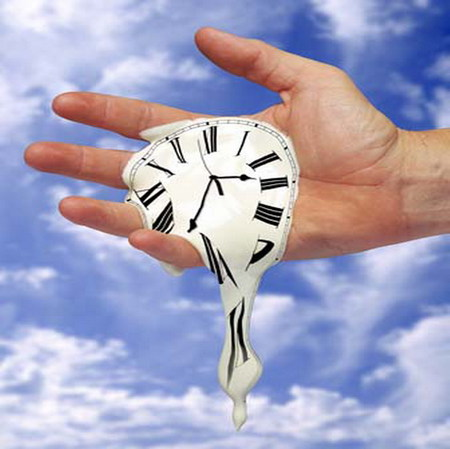
\includegraphics[width=.7\linewidth]{dali}
}

\frame{\frametitle{Plan}
\begin{description}
	\item[Day 1]
	\begin{enumerate}
		\item Origins and milestones of time diary research 

		\item Structure and design of time diary data
\item Computing simple time use estimates
\end{enumerate}
\item [Day 2]
	\begin{enumerate}

\item Tempograms
\item Work schedules
\item Data quality and weighting 

\item Multivariate modelling
\end{enumerate}
\end{description}

}
\frame{\frametitle{Thursday 3 November 2022}

\begin{itemize}

	\item Session 1 2-2.45
\begin{itemize}

\item Origins and milestones of time diary analysis; structure and design of time diary surveys

\item Questions and answers, break
\end{itemize}

	\item Session 2 3-3.45
\begin{itemize}

\item Structure and design of time diary surveys (continued). \item Estimating duration and participation: day- and person-level aggregate statistics

\item Q\&A, break
\end{itemize}

	\item Session 3 4-5
\begin{itemize}

\item Estimating duration and participation (continued)

\item Q\&A; discussion of participants research ideas and interest

         
\end{itemize}
\end{itemize}

}

\frame{\frametitle{How is time studied in sociology?}
\begin{enumerate}
\item Time as an intrinsic object of study
\begin{itemize}
	\item Social theory: ie acceleration (Rosa 2015)
	\item Social times and rhythm (Boulin, Tabbonni)
	\item Rationalisation and modernity: criticisms of the 'clock time' (Southerton)
	\end{itemize}
\item ... As a empirical tool to investigate social issues
\begin{itemize}
	\item Productivity (Organisation studies)
	\item Inequality ie Time poverty/exploitation
	\item  Division of labour within the household
\end{itemize}
\item Long limited by the availability of reliable, systematic empirical  data
\end{enumerate}
}

\frame{\frametitle{Growing  interest from the 20th Century onwards}
	\begin{itemize}
		\item Early 20th Century: peasant households in Russia  \& the Fabians (Women in London) 
		\item Soviet economists: Time Budget of Russian Workers from 1922–1924 (Strumilin); 
		\item US Department for Agriculture time use in farms, towns, and later elite educated “college”, women
		\item In the UK: Mass Observation from 1937 and the BBC listeners surveys
\item Growing acknowledgement of the importance of measuring time in modern societies
	\end{itemize}
}
\frame{\frametitle{What drove this interest for time use?}
	\begin{itemize}
		\item Monitoring economic productivity, in particular household productivity
		\item Labour force / workplace behaviour
		\item Social (central) planning

		\item Better understand consumer behaviour
		\item Investigate social issues ie poverty, gender inequality
		\item More broadly part of continued move towards greater rationalisation of modern societies (Weber)
			\end{itemize}
}

\frame{\frametitle{Contemporary time studies}
\begin{itemize}
\item Large scale mostly Western comparative datasets
\begin{itemize}
\item Alexander Szalai's \textit{The Use of Time}
\begin{itemize}

	\item 12 countries, mostly urban households
	\item First systematic time diary data collection: '\textit{who does what, where, with whom, over 24h}'
	\item Pioneering, remarkable cooperation for the times

\end{itemize}
\item Multinational Time Use Study (MTUS)

\begin{itemize}
	\item J Gershuny at CTUR, UCL
	\item Main source of international harmonised time use data
	\item Large archive: 55 years, 1 million diaries, 30 countries, 70 surveys
\end{itemize}
\item EUROSTAT's Harmonised European Time Use Survey 
\end{itemize}
\item A large number of national studies ie American Time Use Survey; Indian Time Use Survey, etc..

\end{itemize}

}

\frame{\frametitle{What does a typical Time Use survey look like?}
\begin{itemize}
	\item Example: 2015 UK Time Use Survey
	\begin{itemize}

		\item 16,550 diary days of 10,208 respondents in 4,238 households in the UK
				\item Diaries for respondents aged 8 and above 
		\item Collected all year round
			\end{itemize}
		\item Two main components:

	\begin{enumerate}
	
				\item Comprehensive individual survey ie
				
				\begin{itemize}
					\item Socio-demographic characteristics, health, etc..
						\end{itemize}
				\item Time diary 
				\begin{itemize}
					\item 10 minutes time slots
					\item Two days per person (one weekday/one day at the weekend)

				\end{itemize}
	\end{enumerate}
					\item Units of observation are \textit{days }rather than persons

\end{itemize}
	
}
	\frame{\frametitle{What is recorded in time diaries?}
		\begin{itemize}
					\item \textbf{Activities}: main and secondary \small ie 'eating dinner and watching TV'
	
\item \textbf{Location}: \small where the activities took place (ie at home, at work, etc)
\item \textbf{Copresence:} \small who else was present at that time
\item More recently:
\begin{itemize}
\item Whether a device (ie phone, computer, tablet) was used
\item Immediate well-being: enjoyment

\end{itemize}
\item Any combination of the above is an \textit{episode}
\item Activities recoded using a harmonised nomenclature (HETUS)
		\end{itemize}
		
	
}
\frame{\frametitle{A paper time diary }
	\centering
	
\includegraphics[clip,origin=c,width=1.1\linewidth]{pics/UKTUS-diary.png}
	

}



\frame{\frametitle{Common estimates derived from time diaries data}
	\begin{itemize}
	\item The time spent on activities ie their duration
	\item Their sequencing through the day
	\item Whether activities are carried out or not ie their probability.
	\item The importance of activities relative to other activities or other people
	\item Their change over time
		\end{itemize}
}
\frame{\frametitle{Durations of activities }
			\centering

\includegraphics[trim={1cm 8cm 1cm 5cm},clip,width=.9\linewidth]{pics/53_PDFsam_2ND_WhatWeReallyDoAllDay}
			
	\tiny (Source: Gershuny et al 2020)
	}
\frame{\frametitle{Duration of activities?}
	\begin{itemize}
		\item For simplicity, activities were grouped in 4 categories
		\item For each time point, we have the average amount of time spent on each activity
		\item Activities all add up to 24h ie 1,440 minutes.
		\item We can compare time use between groups 
		\item Three main lessons
			\begin{itemize}
			
		\item Overall impression of stability over time
		\item Little change in sleep and leisure duration
		\item Opposite trends in paid and unpaid work
		\item Marked gender differences 
	\end{itemize}
	\end{itemize}
}

\frame{\frametitle{Sequencing of activities through the day -- then... }
	\centering
	\begin{tabular}{cl}
			
\includegraphics[width=.40\pagewidth]{pics/t1961_w}&
\includegraphics[width=.40\pagewidth]{pics/t1961_m}\\

	\end{tabular}
	
	\tiny (Source: Gershuny et al 2020)
}
\frame{\frametitle{Sequencing of activities through the day... And now  }
	\centering
	\begin{tabular}{cl}
		
\includegraphics[width=.4\pagewidth]{pics/t2015_w}&
\includegraphics[width=.4\pagewidth]{pics/t2015_m}\\
		
	\end{tabular}
	
	\tiny (Source: Gershuny et al 2020)
}

\frame{\frametitle{Sequencing of activities}
	\begin{itemize}
		\item These 'tempograms' show by time of the day, the proportion of people engaged in given activities
		\item They provide an overview of daily rhythms:
		\begin{itemize}
			
			\item People busy working between 8 and 6PM
			\item Leisure activity between  6 and 10 PM
			\item Meal times
		\end{itemize}
	\item ... But also social change
		\begin{itemize}
		
		\item The weekdays of men and women have converged over time 
		\item Changes in leisure behaviour
\item Spread of eating time: erosion of the traditional meal
\item Lifestyles have become more diverse
		\end{itemize}

	\end{itemize}
}

\frame{\frametitle{Summary}
\begin{itemize}
\item There has been an increase of interest for the way men, women and households spend their time over the 20th century
\item Systematic time diary data collection from the 1960s
\item There is now large amount of comparative data enabling time use research 
\item Time diaries record primary, secondary activities and their context

\item Stability \textit{and} change in daily behaviour over the last 50 years; gender contrasts

	\end{itemize}
}

\large \frame{\frametitle{2. Time squeeze and acceleration }
	\begin{enumerate}
			\item Are we time-squeezed?
			\item Is time accelerating?
			\item Empirical evidence
	\end{enumerate}
}



\frame{\frametitle{Too many things to do, not enough time?}
	
	\begin{enumerate}
		\item Common trope in the news: 
		\begin{itemize}
			\item '\textit{Too busy to read}' (The Guardian)
			\item \textit{Technology is seeding up our sense of time} (The Telegraph)
			\item \textit{Give up your time to have more time}(The Telegraph)
			\item \textit{Time pressure affects almost every household}  (the Financial Times)
			
		\end{itemize}
		
		
		\item This rings true, but is this supported by empirical evidence?
		
	\end{enumerate}
	
}
\frame{\frametitle{Echoed in sociological research...}
	\begin{itemize}
		\item The overworked American (Schor 1993)
		\begin{itemize}
			\item 'Squirrel cage': work and spend cycle
		\end{itemize}
		
		
		
		\item The time bind (Hochshild 1998)
		\begin{itemize}
			\item People in the US  spend more time on paid work than ever before...
			\item ... Which leaves them with not enough time to fulfil their domestic duties
			\item And feeling dissatisfied, with some ambivalence
		\end{itemize}
		\item Abundant empirical literature on work life balance/conflict
	\end{itemize}
	
}	
\frame{\frametitle{Is time accelerating?}
	
	\begin{itemize}
		\item Acceleration (Rosa 2003)
		\begin{itemize}
			\item Technological acceleration (communication, transport \& production) quest for speed in advanced capitalist societies;
			\item Acceleration of social change 
			\item Acceleration of the pace of life
		\end{itemize}
		
		\item Harriedness (Southerton et al 2005)
		\begin{itemize}
			\item Volume ie duration
			\item Fragmentation/disorganisation: work schedules
			\item Temporal density of work and leisure
		\end{itemize}
	\end{itemize}
	
}


\frame{\frametitle{What can we make of this?}
	\begin{itemize}
		\item Little evidence of overall working time increase
		\begin{itemize}
			\item ... But differences between groups may cancel each other
		\end{itemize}
		\item Parenting ideals: hyperparenting
		\item Dual earners, high pressured professional  families may have greater public visibility
		\item 'Busyness' as badge of honour (Gershuny)?
	\end{itemize}
}

%\frame{\frametitle{Time stress and income \small(Hamermesh \& Lee 2007)}
%	\begin{itemize}
%		\item 	Working time positively related to stress
%		\item ... But people reporting higher levels of  stress tend to be higher earners
%	\end{itemize}
%	
%	\begin{tabular}{cc}
%		Male&Female\\
%		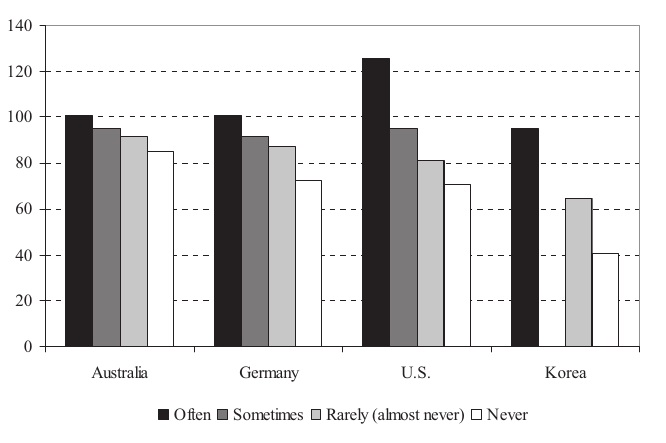
\includegraphics[width=0.5\textwidth]{tpress_m}&		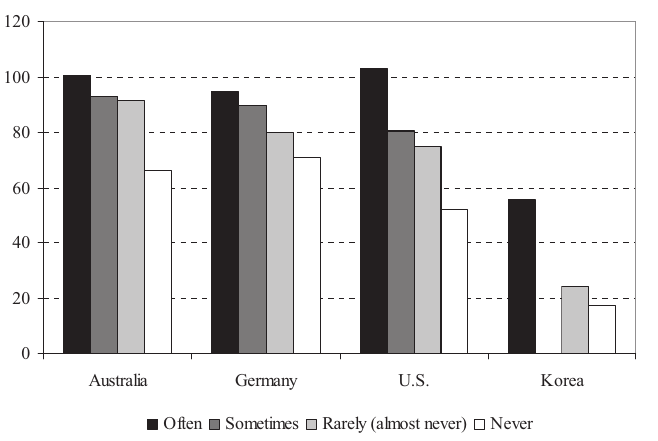
\includegraphics[width=0.5\textwidth]{tpress_f}\\
%	\end{tabular}
%}

\frame{\frametitle{Time fragmentation \small (Gershuny \& Sullivan 2016)}
	\begin{tabular}{c}
		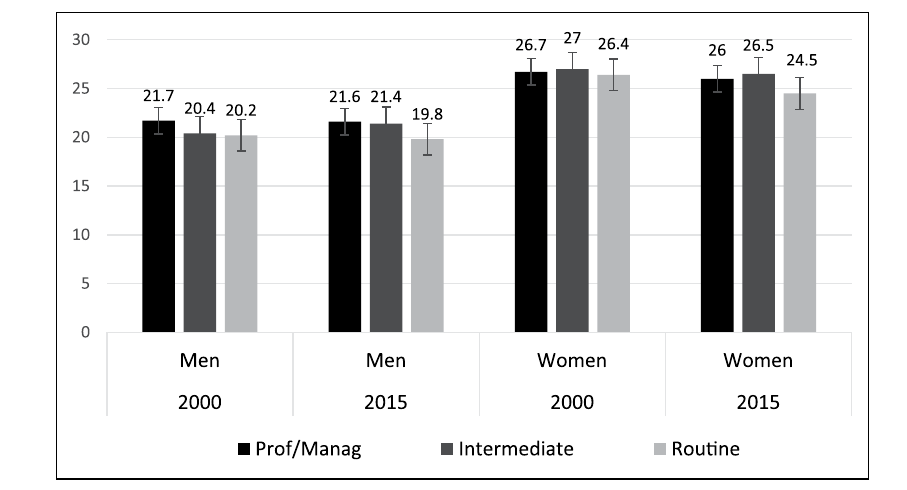
\includegraphics[width=0.8\textwidth]{fragm}\\
	\end{tabular}
	\begin{itemize}
		\item \small  Number of activities by gender and social class, UK 2015.
		\item Few differences in the number of activities
		
	\end{itemize}
	
}

\frame{\frametitle{... Multitasking \small (Gershuny \& Sullivan 2016)}
	\begin{tabular}{c}
		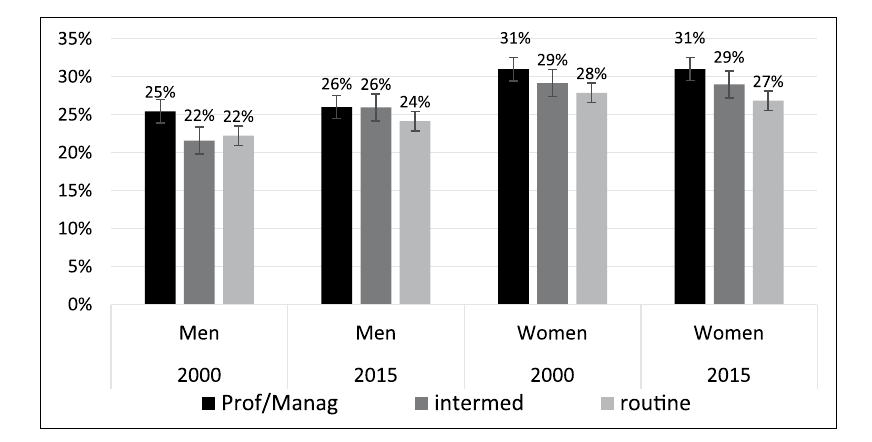
\includegraphics[width=0.8\textwidth]{multit}\\
	\end{tabular}
	\begin{itemize}
		\item \small  \% of daily activities multitasked, by gender and social class, UK 2015.
		\item Differences are small
		
	\end{itemize}
	
}

\frame{\frametitle{Device use \& stress \small (Gershuny \& Sullivan 2016)}
	\begin{tabular}{c}
		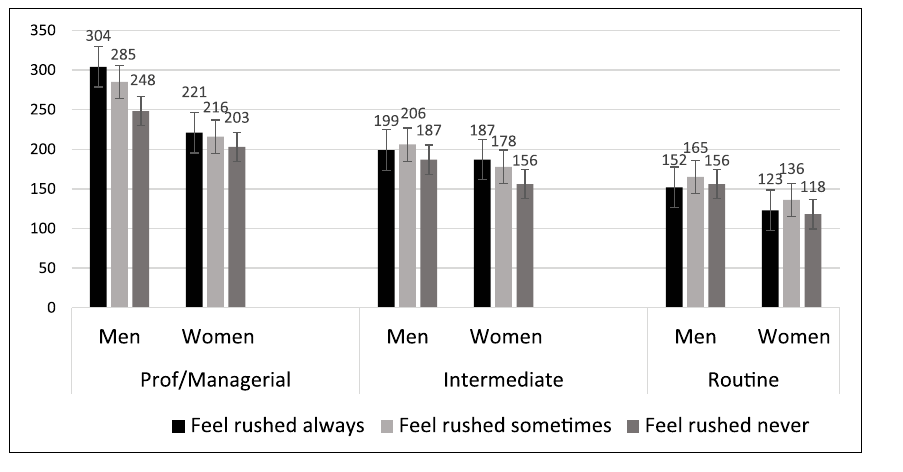
\includegraphics[width=0.8\textwidth]{ictstress}\\
	\end{tabular}
	\begin{itemize}
		\item \small  Number of activities by gender, social class and feeling rushed: UK 2015.
		
		\item Professional and managerial who always feel rushed report more time using devices.
		
	\end{itemize}
	
}

\frame{\frametitle{Summary}
	\begin{itemize}
		\item Report of acceleration of pace of life and scarceness of time 
		\item Matched by an increased sense of being rushed
		\item Little systematic empirical evidence that overall working time, multitasking and fragmentation have increased
		\item But use of IT device is associated with feeling rushed.
		\item Expectation about childcare and leisure may have raised
	\end{itemize}
}

\end{document}




